% 实验结果分析：阅读说明修订稿；全部图表均已内嵌。
% 导言区依赖：amsmath、amssymb、graphicx、float、array、booktabs、longtable、url。
% 图片路径为 figures/；不要与“问题一_全部表格.tex”重复载入。
\subsection{实验结果分析}
\label{sec:p1_results}
\urlstyle{same}

本节从观测覆盖、对齐筛选和结果回溯三个方面检查特征输出。首先确认全部样本是否完成处理，并区分“生成了特征记录”与“获得了有效面部观测”；随后结合词级置信度和片段级文本差异，确定候选时间区间的使用范围。在此基础上，通过固定窗口对照考察时间划分对特征变化与词区间完整性的影响，再用人工审核解释整段异常，最后以典型样本展示词与视听记录之间的映射。本问未训练情感预测模型，因此以下结果评价特征提取与时序组织，不涉及情感分类准确率。

\subsubsection{样本覆盖完整性与特征有效性}
\label{sec:p1_quality_scope}

100条样本均生成三种模态的词级特征矩阵，矩阵行数与各自原文词数一致，共保留1932个词位置，未发生截断。表~\ref{tab:p1_result_overview}汇总处理范围及观测覆盖情况：文本与声学在全部词位置均有可用于计算的记录，视觉观测则存在缺失。表中样本比例以100为分母，词比例以1932为分母，各行不构成互斥分类。

\begin{table}[H]
    \centering\small
    \caption{样本处理与三种模态的观测覆盖情况}
    \label{tab:p1_result_overview}
    \setlength{\tabcolsep}{6pt}
    \renewcommand{\arraystretch}{1.12}
    \ifdefined\pOneCompactTableBox\else\newsavebox{\pOneCompactTableBox}\fi
    \begin{lrbox}{\pOneCompactTableBox}
    \begin{tabular}{lrr}
        \toprule
        统计项目 & 数量 & 占比\\
        \midrule
        已处理样本 & 100 & 100.00\%\\
        与原文对应的输出词位置 & 1932 & 100.00\%\\
        文本模态可观测的词 & 1932 & 100.00\%\\
        声学模态可观测的词 & 1932 & 100.00\%\\
        视觉模态可观测的词 & 1595 & 82.56\%\\
        \bottomrule
    \end{tabular}
    \end{lrbox}
    \usebox{\pOneCompactTableBox}
\par\smallskip
\end{table}

图~\ref{fig:p1_observation_summary}将视觉缺失与声学低能量放在同一组图中，分别检查两种模态的输入状态。图(a)的上、下两行分别以抽样帧和候选词区间为统计单位：3973帧中有3253帧获得面部特征，720帧未获得可用结果；聚合到词位置后，1595个词具有有效面部记录，337个词缺少相应记录。一个词可以关联多帧，一帧也可能参与多个词的聚合，因此两行比例的分母不同，不能解释为聚合前后的准确率变化。

图(b)检查声学记录的幅度状态。以数字音频满幅1为基准，将短时均方根幅度（RMS）低于0.0031623的记录标记为低能量，77261条声学记录中共有9918条满足该条件，占12.84\%。这里的低能量表示波形幅度较小，不能直接作为无语音或观测缺失的判据。

\begin{figure}[H]
    \centering
    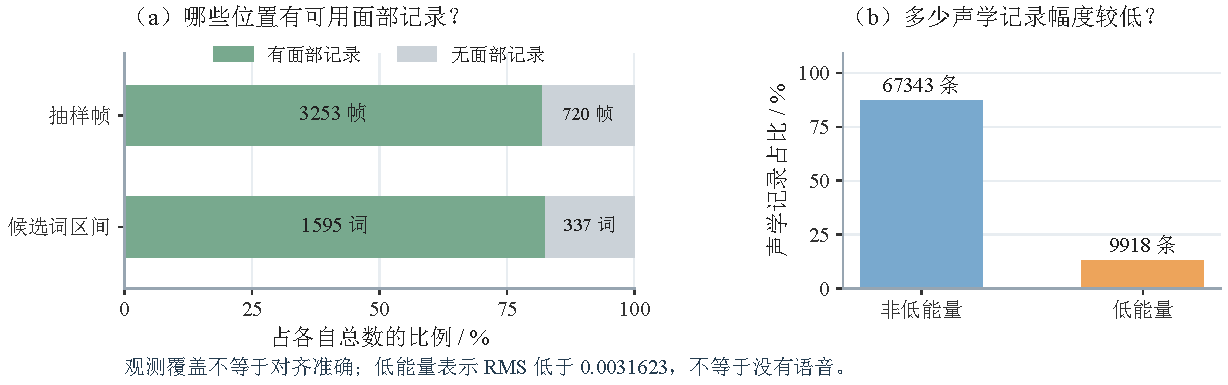
\includegraphics[width=\linewidth]{figures/fig_p1_observation_summary.pdf}
    \caption{模态观测检查：面部记录的覆盖范围与声学记录的低能量占比}
    \label{fig:p1_observation_summary}
    \label{fig:p1_visual_coverage}
    \label{fig:p1_audio_energy_share}
\end{figure}

为说明低能量标记在时间轴上的含义，图~\ref{fig:p1_rms_explained}展示样本\nolinkurl{-iRBcNs9oI8$_$9}的333条RMS记录，其中147条低于阈值。图(a)显示完整幅度范围，图(b)保持相同横轴，仅放大纵轴接近零的部分；橙色虚线为阈值，橙点为低能量记录。两图结合可见，该样本既包含较强的幅度峰值，也包含持续的低幅度区间，因而不能用一个整段平均值替代局部记录的检查。

\begin{figure}[H]
    \centering
    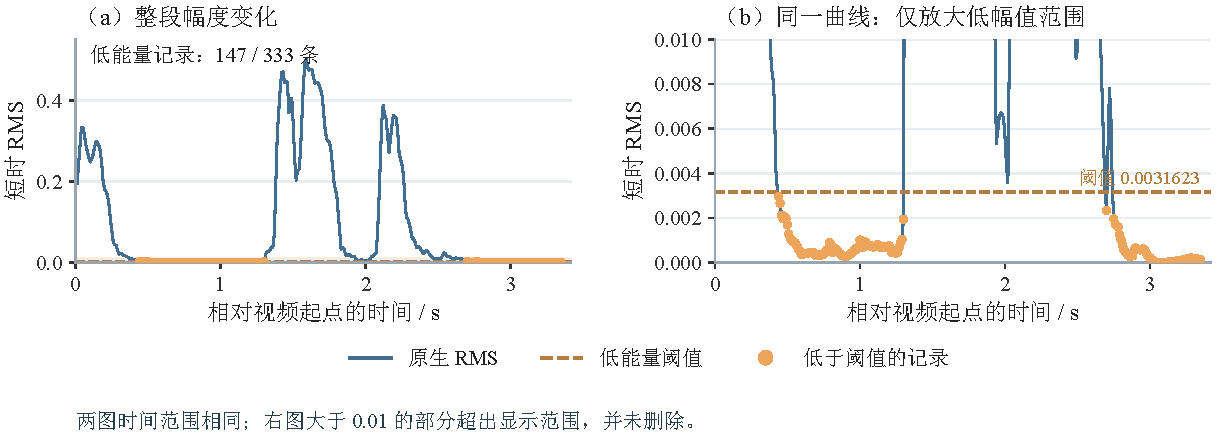
\includegraphics[width=\linewidth]{figures/fig_p1_rms_explained.pdf}
    \caption{同一样本的短时RMS及低幅值放大：橙点表示低于阈值的记录}
    \label{fig:p1_rms_explained}
    \label{fig:p1_rms}
    \label{fig:p1_rms_zoom}
\end{figure}

此外，两条样本的解码音频波形全为零，对应声学特征各维均不随时间变化。这说明“具有可计算的声学记录”不等于“包含与转写对应的语音”。观测覆盖检查之后，还需要判断给定转写能否在实际音频中得到支持。

\subsubsection{时序对齐质量评估与人工审核}
\label{sec:p1_timing_quality}

CTC强制对齐为1932个词均生成候选时间区间，但满足字符路径约束并不保证真实词界准确。本文先从局部词匹配和整段文本差异两个层次进行诊断，再汇总筛选后的词位置范围。

词级置信度取最优CTC路径中属于该词的文字字符帧概率的几何平均，不含空白符和词界符，用于描述模型对局部匹配的支持程度。片段级诊断词错误率（Word Error Rate，WER）则先获取无转写约束的贪心识别文本，再计算其与规范化转写之间的最少词编辑数，并除以参考词数。WER较大表示两份文本差异较大；由于编辑数包含插入操作，其值可以超过1。两项指标来自同一声学模型，均不构成独立的词界准确性验证。

图~\ref{fig:p1_alignment_screening}(a)以1932个词为统计对象。置信度中位数为0.9585，1034个词不低于0.95，但0.1阈值左侧仍有350个词，说明较高的整体得分不能排除局部匹配异常。图(b)以100条片段为统计对象，诊断WER均值为0.4689，0.8阈值右侧有21条片段，其中9条超过1。两幅图的阴影区域分别提示需要关注的低置信度词和文本差异较大的片段。

\begin{figure}[H]
    \centering
    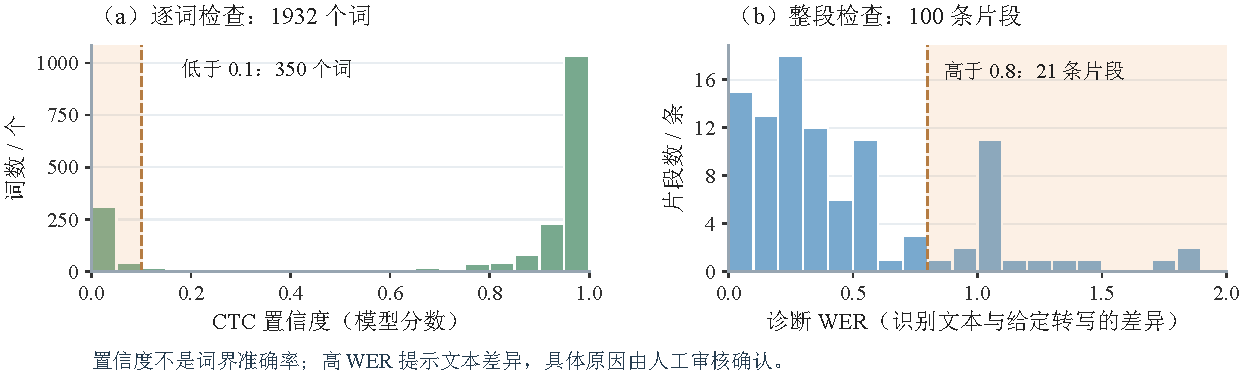
\includegraphics[width=\linewidth]{figures/fig_p1_alignment_screening.pdf}
    \caption{对齐诊断的两个层次：逐词匹配支持与整段文本差异}
    \label{fig:p1_alignment_screening}
    \label{fig:p1_ctc_confidence}
    \label{fig:p1_diagnostic_wer}
\end{figure}

据此，本文实施片段级与逐词两层筛选。片段级条件为：平均词置信度低于0.2、置信度低于0.1的词超过一半、诊断WER大于0.8，或无法形成完整CTC路径；满足任一条件即列入整段复核，暂不采用其词级时间对应。在其余样本中，仅将成功获得候选起止时间且置信度不低于0.1的词计为通过筛选。阈值是在检查实际异常后设定的保守条件，未利用情感标签或人工词界标注优化。

图~\ref{fig:p1_quality_flow}将两层筛选与模态观测检查串联起来。在100条样本中，19条的平均词置信度低于0.2，20条有超过一半的词置信度低于0.1，21条的诊断WER大于0.8，没有样本因无法形成完整CTC路径而被标记。这四项条件分别检查，每条样本只要满足其中任一项就进入整段复核；同一样本可能同时满足多项条件，因此各项数量不能直接相加。本次前两项标记的样本均已包含在WER大于0.8的21条样本中，去除重复计数后，需整段复核的仍为21条，共涉及317个词。其余79条样本包含1615个词，其中70个因置信度不足未通过逐词筛选，剩余1545个通过筛选，占全部词的79.97\%。这1545个词中，158个缺少有效面部记录，1387个同时满足对齐筛选和三模态可观测条件，占全部词的71.79\%。

\begin{figure}[H]
    \centering
    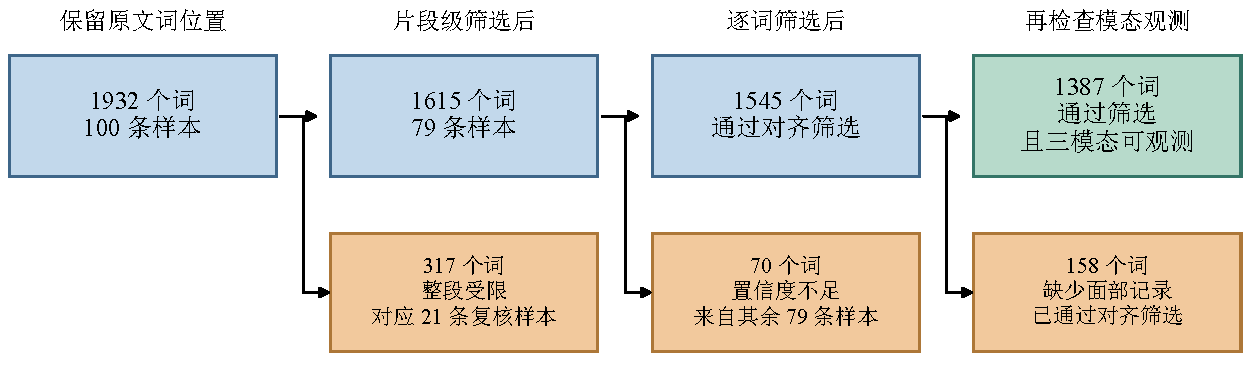
\includegraphics[width=\linewidth]{figures/fig_p1_quality_flow.pdf}
    \caption{从全部词位置到满足不同使用条件的词位置：各分支数量可逐项核对}
    \label{fig:p1_quality_flow}
\end{figure}

图中橙色分支表示未满足当前检查条件的词，原文、特征及候选时间仍全部保留。其中，317个整段受限词包含37个局部置信度达到阈值的词，这也解释了为何未通过对齐筛选的387个词多于低置信度词的350个：片段级文本差异可能限制局部得分较高的词。

进一步将片段平均置信度阈值取0.1、0.2、0.3，诊断WER阈值取0.6、0.8、1.0，其余条件保持不变。在三种平均置信度阈值下，待复核样本数均随WER阈值变化依次为25、21、20条，表明当前数据的复核数量主要受WER条件影响。该检查反映筛选范围对阈值的敏感性，不能据此确定最优阈值或计算真实对齐准确率。

\label{sec:p1_window_analysis}
确定候选词区间的筛选范围后，进一步考察时间划分会怎样改变特征表示。本文在相同原生特征上构造0.2~s和0.5~s固定窗口，窗口从零时刻开始，末窗截取至片段终点，视听特征沿用有效时间交叠加权规则。该对照同时关注两个方面：平均聚合后还保留多少局部变化，以及固定边界是否将一个词对应的时间区间分散到多个窗口。

图~\ref{fig:p1_window_experiment}上方给出处理步骤：先保留原生记录，再分别按两种窗口聚合，最后依据时间交叠关系将窗口特征映回原生记录位置。图(a)以响度为例，灰线为原生记录，蓝线和橙线分别为短窗与长窗聚合后的重建结果。原生曲线中的局部峰谷在平均后被削弱，较长窗口的平滑范围更大。这里的“重建”指从窗口特征近似还原原生特征序列，不是重建原始音频。

图(b)检查同一样本中的词区间是否被固定窗口切分。绿色线为\texttt{successful}的候选区间$[1.84247,2.40247]\,\mathrm{s}$，上、下两排分别为0.2~s和0.5~s窗口。该词分别与4个短窗和2个长窗交叠，在两种划分下均计为一个跨界词。第四个短窗的交叠仅约0.00247~s，图中以箭头注明；统计时将大于$10^{-8}\,\mathrm{s}$的交叠视为有效交叠。跨界指标只判断是否与至少两个窗口交叠，不区分交叠窗口数量及切分幅度。

上述图示采用样本\nolinkurl{-egA8-b7-3M$_$1}。其选取条件为未触发整段复核、面部观测帧占比不低于80\%，且时长最接近10~s。该样本实际时长10.266~s，包含20个词，其中18个通过对齐筛选。

\begin{figure}[H]
    \centering
    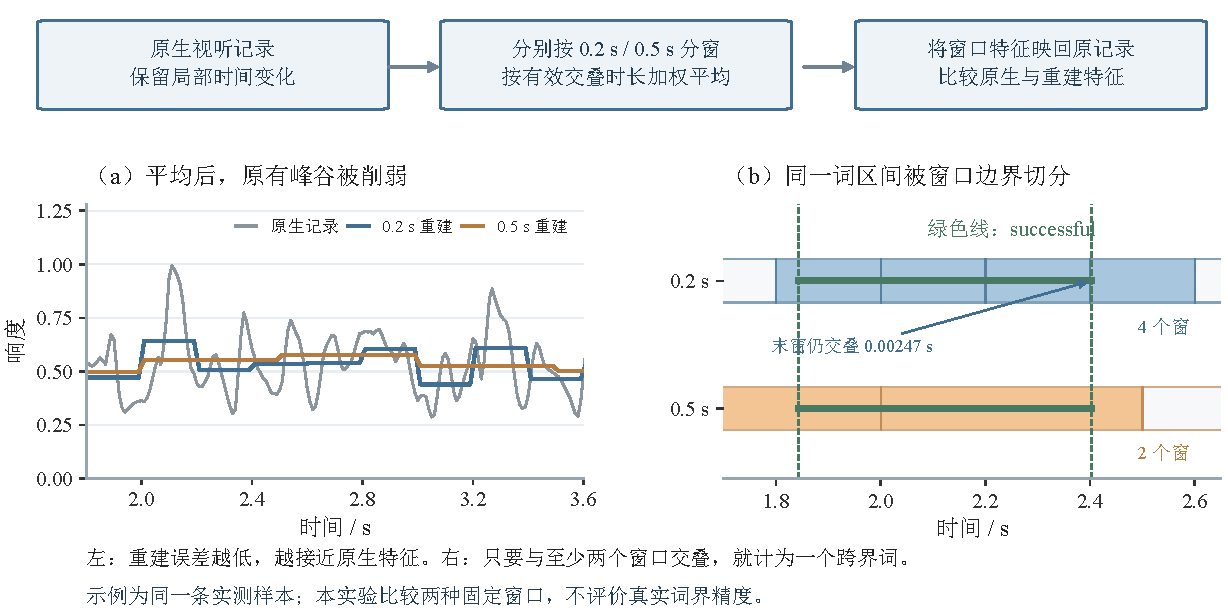
\includegraphics[width=\linewidth]{figures/fig_p1_window_experiment.pdf}
    \caption{固定窗口对照的操作与实例：特征平均削弱峰谷，窗口边界可能切分词区间}
    \label{fig:p1_window_experiment}
    \label{fig:p1_window_reconstruction}
    \label{fig:p1_word_window_overlap}
\end{figure}

为将实例现象推广到全量样本，本文采用标准化重建均方误差和词跨界比例进行评价。前者将重建特征与原生特征之差按各维原生标准差归一化，再对有效记录和维度的平方误差取平均，数值越低表示越接近原生特征。计算仅纳入标准差大于$10^{-6}$的维度；有记录但全部维度恒定时记0，无有效记录时不计入模态均值。后者在每条样本通过对齐筛选的词中，统计跨越窗口边界的词所占比例，数值越高表示被切分的词越多。两类指标均先在样本内计算，再对相应有效样本等权平均。

图~\ref{fig:p1_window_tradeoff}汇总全量对照。图(a)、(b)中的短窗箱体整体低于长窗箱体，声学平均重建误差由0.7467降至0.5449，视觉由0.4373降至0.2357，相对降幅分别为27.02\%和46.10\%。图(c)则呈相反方向，平均词跨界比例由39.50\%升至71.33\%，增加31.83个百分点。三幅图分别基于100条声学样本、87条具有有效面部记录的样本和79条未触发整段复核的样本。图中菱形标出均值，箱内横线标出中位数，箱体覆盖第25至第75百分位数，须线延伸至1.5倍四分位距内的最远观测；箱外圆点仍参与统计。

\begin{figure}[H]
    \centering
    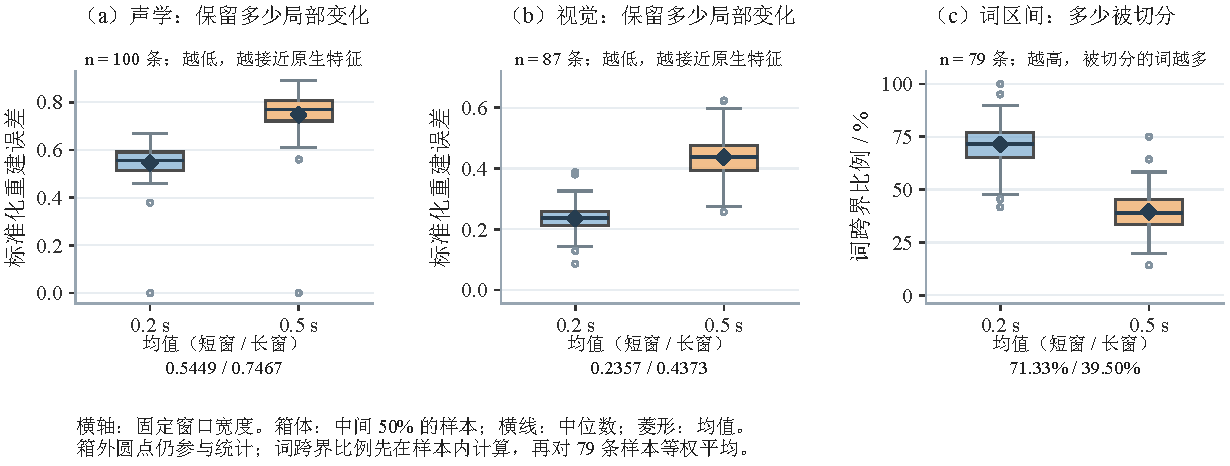
\includegraphics[width=\linewidth]{figures/fig_p1_window_tradeoff.pdf}
    \caption{两种固定窗口的全量对照：短窗重建误差较低，同时词跨界比例较高}
    \label{fig:p1_window_tradeoff}
    \label{fig:p1_audio_window_error}
    \label{fig:p1_vision_window_error}
    \label{fig:p1_word_crossing_ratio}
\end{figure}

逐样本比较进一步表明，98条样本的短窗声学误差更低，另2条相同；87条样本的短窗视觉误差均更低；77条样本的短窗词跨界比例更高，另2条相同。两条声学误差相同的样本即前述全零音频样本，其特征不随时间变化，两种窗口的误差均按规则记0。将这两条样本单独列出后，其余98条样本的短窗、长窗平均声学误差分别为0.5560和0.7619，差异方向保持一致。

因此，本次固定窗口对照揭示了局部变化保留与词区间完整性之间的权衡：较短窗口更接近原生特征变化，同时有更多词区间被窗口边界切分。该结果仅比较两种固定窗口，不能据此断言词级表示具有更低重建误差、更准确词界或更高情感预测性能。

自动诊断确定了需要复核的片段，固定窗口对照说明了时间划分的影响；对于21条整段受限样本，还需要检查其异常是否源于输入内容不对应。为此，本文对照实际音频与给定英文转写进行人工审核，按主要问题划分为五类，见表~\ref{tab:p1_manual_review}。各类互不重叠，共涉及317个原文词。

\begin{table}[H]
    \centering\small
    \caption{21条复核样本的人工审核结果}
    \label{tab:p1_manual_review}
    \setlength{\tabcolsep}{6pt}
    \renewcommand{\arraystretch}{1.12}
    \ifdefined\pOneCompactTableBox\else\newsavebox{\pOneCompactTableBox}\fi
    \begin{lrbox}{\pOneCompactTableBox}
    \begin{tabular}{lcc>{\raggedright\arraybackslash}p{18em}}
        \toprule
        审核发现 & 样本数 & 原文词数 & 主要表现\\
        \midrule
        音轨与文本不对应 & 11 & 120 & 实际语音内容与给定转写不对应\\
        无对应朗读 & 5 & 64 & 未听到对应朗读，其中1条为音乐\\
        非英语语音 & 3 & 93 & 实际语音并非英语\\
        分段内容不对应 & 1 & 18 & 前半段无朗读，后半段语音与转写不对应\\
        音频卡顿、局部对应 & 1 & 22 & 音频存在卡顿，部分词语与文本一致，但未形成完整对应\\
        \midrule
        合计 & 21 & 317 & \\
        \bottomrule
    \end{tabular}
    \end{lrbox}
    \usebox{\pOneCompactTableBox}
\end{table}

审核发现，音轨与文本不对应、缺少对应朗读等情况使给定转写缺少相应的语音依据；非英语语音则与所用英语声学模型及英文对齐目标不匹配。其中，3条非英语样本均来自视频\nolinkurl{-yRb-Jum7EQ}，两条全零音频样本归入“无对应朗读”。这些异常具有不同来源，不能统一解释为词界定位偏差。

样本\nolinkurl{-HwX2H8Z4hY$_$9}还说明了片段级检查的必要性。其平均词置信度为0.7238，仅9.09\%的词低于0.1，但诊断WER达到0.8636。人工审核发现音频存在卡顿，部分词语与转写一致，却没有形成完整逐词对应，说明局部得分较高不足以确认整段对应关系。

依据审核结果，本文维持这21条样本整体词级对应受限的标记。审核未重建人工词界，因此不恢复局部词的对齐标记，前述筛选数量保持不变。此次审核只覆盖自动筛出的21条样本，不能据此认定其余79条均无异常，也不能计算全量词界准确率；逐样本审核说明随结果附件保存。

\subsubsection{典型样本的跨模态时序对齐验证}
\label{sec:p1_verification_examples}

在明确使用条件后，本节继续使用\nolinkurl{-egA8-b7-3M$_$1}，检查一个词能否回溯至相应的音频记录和实际画面。图~\ref{fig:p1_multimodal_result}自上而下排列视频帧、候选词区间、响度和面部系数，所有时间均相对于视频起点。阅读时先选定一个词，再沿候选边界向下查看相应时段的视听记录；浅绿底突出\texttt{successful}，其区间内约2.11~s处出现响度峰值。上方图片按标注时刻定位，图片宽度不代表持续时间；面部曲线的数据点对应抽样帧，连线仅辅助观察。

\begin{figure}[H]
    \centering
    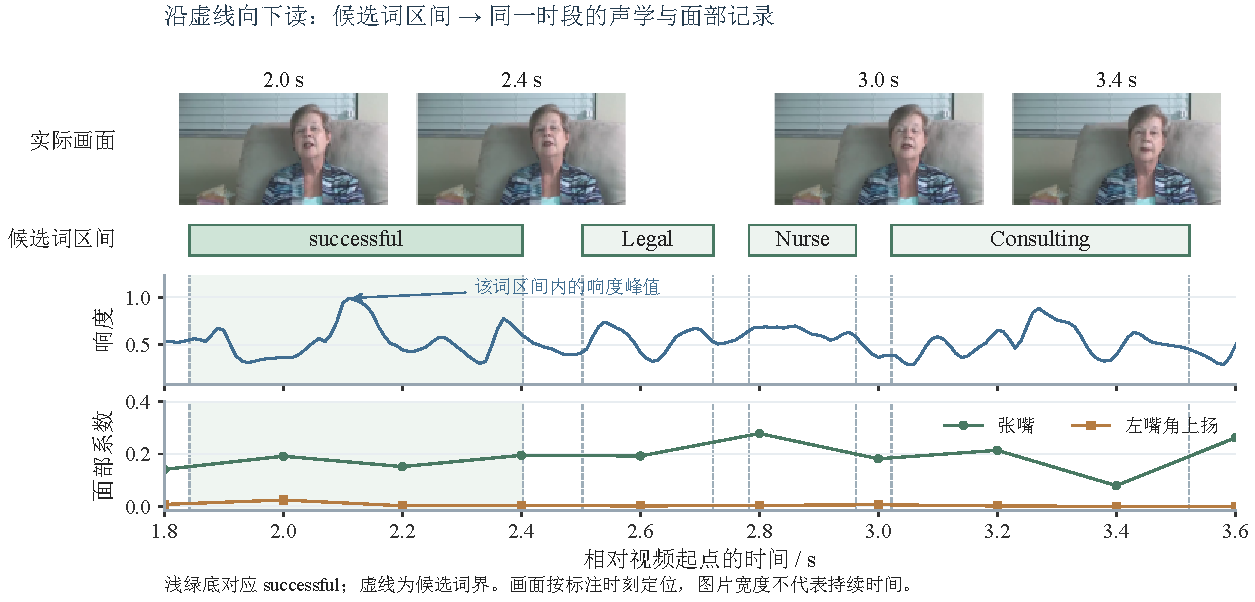
\includegraphics[width=\linewidth]{figures/fig_p1_multimodal_readable.pdf}
    \caption{词级映射的回溯示例：从候选词区间定位同一时段的声音与画面}
    \label{fig:p1_multimodal_result}
\end{figure}

表~\ref{tab:p1_mapping_records}列出部分映射记录。以\texttt{successful}为例，其候选区间为$[1.8425,2.4025]\,\mathrm{s}$，文本表示对应子词索引3，声学表示由183--240号共58条原生记录聚合，视觉表示由1.8、2.0、2.2、2.4~s四帧聚合。索引从0开始；声学索引指特征记录，而非波形采样点。视觉帧根据其时间支持区间参与聚合，因此帧中心可以位于词区间之外。边界帧仅部分覆盖词区间，其聚合权重相应较小。

\begin{table}[H]
    \centering\small
    \caption{典型样本的部分词级映射记录}
    \label{tab:p1_mapping_records}
    \setlength{\tabcolsep}{6pt}
    \renewcommand{\arraystretch}{1.12}
    \ifdefined\pOneCompactTableBox\else\newsavebox{\pOneCompactTableBox}\fi
    \begin{lrbox}{\pOneCompactTableBox}
    \begin{tabular}{lcccc}
        \toprule
        原文词 & 子词索引 & 候选区间/s & 声学记录索引 & 视觉帧时刻/s\\
        \midrule
        started & 1 & $[1.2825,1.6425]$ & 127--164 & 1.2, 1.4, 1.6\\
        successful & 3 & $[1.8425,2.4025]$ & 183--240 & 1.8, 2.0, 2.2, 2.4\\
        Consulting & 6 & $[3.0225,3.5225]$ & 301--352 & 3.0, 3.2, 3.4, 3.6\\
        \bottomrule
    \end{tabular}
    \end{lrbox}
    \usebox{\pOneCompactTableBox}
\par\smallskip
\parbox{\wd\pOneCompactTableBox}{\footnotesize 注：索引从0开始；声学索引指具有正聚合权重的原生特征记录，不是波形采样点。视觉帧按其时间支持区间与候选词区间的交叠关系参与聚合，帧中心不必位于词区间内部。}
\end{table}

图表共同说明了词级输出如何回到原生记录，但映射可追溯并不直接证明候选词界准确。为核验计算过程，本文对全部样本的交叠权重、视听聚合值和CTC置信度进行独立复算，重新计算诊断WER，并解码音视频核对时间记录与低能量标记；100条样本在既定数值容差内均与保存结果一致。该检查验证输出遵循既定计算规则，真实词界精度仍需人工时间标注评价。典型样本中的\texttt{in}和\texttt{1989}仍因置信度不足未通过逐词筛选，进一步表明整段未触发复核并不意味着其中所有词均可用于对齐分析。

\subsubsection{三模态特征文件说明与100条样本结果汇总}
\label{sec:p1_delivery}

为便于逐样本查阅，表~\ref{tab:p1_feature_specification}汇总三种模态的输出规格，表~\ref{tab:p1_all_samples}按词级对应的使用范围分组，列出全部100条样本的编号、时长、词数与有效位置统计。各组划分依据前述观测状态、对齐筛选和人工审核结果，高维特征的具体数值保存在对应文件中。

\begin{table}[H]
    \centering\small
    \caption{三种模态的词级特征规格}
    \label{tab:p1_feature_specification}
    \setlength{\tabcolsep}{6pt}
    \renewcommand{\arraystretch}{1.12}
    \ifdefined\pOneCompactTableBox\else\newsavebox{\pOneCompactTableBox}\fi
    \begin{lrbox}{\pOneCompactTableBox}
    \begin{tabular}{lccc}
        \toprule
        模态 & 特征维数 & 样本矩阵形状 & 对齐粒度\\
        \midrule
        文本 & 768 & $L\times768$ & 原文词\\
        声学 & 25 & $L\times25$ & 原文词\\
        视觉（面部） & 52 & $L\times52$ & 原文词\\
        \bottomrule
    \end{tabular}
    \end{lrbox}
    \usebox{\pOneCompactTableBox}
\par\smallskip
\parbox{\wd\pOneCompactTableBox}{\footnotesize 注：$L$为对应样本的原文词数。各样本按实际词数存储，填充数与截断词数均为0；视觉模态不可观测的词位置采用零向量占位，并附无效标记。}
\end{table}

全量表中，“原文词数”对应三个矩阵的行数，“视觉可观测词数”统计能够聚合有效面部记录的词，“通过对齐筛选词数”采用前述两层筛选条件，最后一列统计通过筛选且三种模态均可观测的词数。由于文本与声学在全部词位置均有可计算记录，最后一列等于通过对齐筛选与视觉可观测两个条件的交集。片段时长与音频时长采用实际解码记录，不表示有效语音或面部信息的累计时长。

例如，样本-s9qJ7ATP7w\$\_\$7共有28个词，其中14个视觉可观测，24个通过对齐筛选，同时满足两项条件的有12个。交集数量不能取前两项数量的较小值代替。

按上述口径，32条样本的全部词通过筛选且三种模态均可观测，46条样本仅部分词满足两项条件，1条样本的全部词通过对齐筛选但视觉模态不可观测，另21条样本经人工审核后整体词级对应仍受限。全量表按这四类依次排列，已审核的21条样本统一归入最后一类，各组互不重叠。

\begingroup
\small
\setlength{\tabcolsep}{6pt}
\renewcommand{\arraystretch}{1.12}
\setlength{\LTleft}{\fill}
\setlength{\LTright}{\fill}
\begin{longtable}{lrrrrrr}
\caption{附件1全部样本的特征输出与有效位置统计}\label{tab:p1_all_samples}\\
\toprule
样本编号 & \shortstack{片段\\时长/s} & \shortstack{音频\\时长/s} & \shortstack{原文\\词数} & \shortstack{视觉可观测\\词数} & \shortstack{通过对齐\\筛选词数} & \shortstack{其中三种模态\\都可观测\\词数}\\
\midrule
\endfirsthead
\multicolumn{7}{c}{表~\thetable\quad 特征输出与有效位置统计（续）}\\
\toprule
样本编号 & \shortstack{片段\\时长/s} & \shortstack{音频\\时长/s} & \shortstack{原文\\词数} & \shortstack{视觉可观测\\词数} & \shortstack{通过对齐\\筛选词数} & \shortstack{其中三种模态\\都可观测\\词数}\\
\midrule
\endhead
\midrule
\multicolumn{7}{r}{续下页}\\
\endfoot
\bottomrule
\endlastfoot
\multicolumn{7}{l}{\textbf{1. 全部词通过筛选且三种模态都可观测（32条）}}\\*
\nolinkurl{-3g5yACwYnA$_$3} & 14.389 & 14.328 & 29 & 29 & 29 & 29\\
\nolinkurl{-3nNcZdcdvU$_$5} & 7.868 & 7.789 & 18 & 18 & 18 & 18\\
\nolinkurl{-6rXp3zJ3kc$_$8} & 12.805 & 12.738 & 34 & 34 & 34 & 34\\
\nolinkurl{-I_e4mIh0yE$_$1} & 7.622 & 7.444 & 18 & 18 & 18 & 18\\
\nolinkurl{-I_e4mIh0yE$_$3} & 9.163 & 8.994 & 22 & 22 & 22 & 22\\
\nolinkurl{-MeTTeMJBNc$_$0} & 9.333 & 9.218 & 21 & 21 & 21 & 21\\
\nolinkurl{-MeTTeMJBNc$_$13} & 5.430 & 5.255 & 14 & 14 & 14 & 14\\
\nolinkurl{-RfYyzHpjk4$_$11} & 5.239 & 5.075 & 17 & 17 & 17 & 17\\
\nolinkurl{-RfYyzHpjk4$_$8} & 4.589 & 4.532 & 17 & 17 & 17 & 17\\
\nolinkurl{-UUCSKoHeMA$_$0} & 7.867 & 7.732 & 18 & 18 & 18 & 18\\
\nolinkurl{-UacrmKiTn4$_$10} & 7.362 & 7.242 & 18 & 18 & 18 & 18\\
\nolinkurl{-UacrmKiTn4$_$4} & 4.741 & 4.682 & 14 & 14 & 14 & 14\\
\nolinkurl{-aNfi7CP8vM$_$7} & 8.695 & 8.538 & 18 & 18 & 18 & 18\\
\nolinkurl{-aqamKhZ1Ec$_$0} & 11.000 & 10.890 & 14 & 14 & 14 & 14\\
\nolinkurl{-dxfTGcXJoc$_$1} & 16.161 & 16.018 & 37 & 37 & 37 & 37\\
\nolinkurl{-egA8-b7-3M$_$16} & 5.538 & 5.483 & 11 & 11 & 11 & 11\\
\nolinkurl{-egA8-b7-3M$_$17} & 7.271 & 7.095 & 16 & 16 & 16 & 16\\
\nolinkurl{-egA8-b7-3M$_$18} & 8.386 & 8.266 & 22 & 22 & 22 & 22\\
\nolinkurl{-egA8-b7-3M$_$20} & 6.645 & 6.474 & 20 & 20 & 20 & 20\\
\nolinkurl{-egA8-b7-3M$_$26} & 6.031 & 5.921 & 15 & 15 & 15 & 15\\
\nolinkurl{-egA8-b7-3M$_$6} & 6.265 & 6.183 & 12 & 12 & 12 & 12\\
\nolinkurl{-egA8-b7-3M$_$9} & 5.090 & 4.936 & 10 & 10 & 10 & 10\\
\nolinkurl{-mqbVkbCndg$_$0} & 6.500 & 6.386 & 14 & 14 & 14 & 14\\
\nolinkurl{-s9qJ7ATP7w$_$6} & 2.475 & 2.315 & 5 & 5 & 5 & 5\\
\nolinkurl{-s9qJ7ATP7w$_$8} & 3.295 & 3.184 & 12 & 12 & 12 & 12\\
\nolinkurl{-t217m2on-s$_$7} & 17.183 & 17.026 & 45 & 45 & 45 & 45\\
\nolinkurl{-tPCytz4rww$_$10} & 4.789 & 4.679 & 12 & 12 & 12 & 12\\
\nolinkurl{-tPCytz4rww$_$11} & 5.467 & 5.379 & 17 & 17 & 17 & 17\\
\nolinkurl{-tPCytz4rww$_$18} & 6.645 & 6.569 & 16 & 16 & 16 & 16\\
\nolinkurl{-uywlfIYOS8$_$4} & 6.045 & 5.881 & 18 & 18 & 18 & 18\\
\nolinkurl{-wny0OAz3g8$_$0} & 3.333 & 3.274 & 9 & 9 & 9 & 9\\
\nolinkurl{-wny0OAz3g8$_$2} & 6.687 & 6.523 & 23 & 23 & 23 & 23\\
\addlinespace[0.5em]
\multicolumn{7}{l}{\textbf{2. 部分词通过筛选且三种模态都可观测（46条）}}\\*
\nolinkurl{-3g5yACwYnA$_$13} & 5.514 & 5.399 & 15 & 15 & 14 & 14\\
\nolinkurl{-3g5yACwYnA$_$2} & 9.394 & 9.231 & 14 & 14 & 13 & 13\\
\nolinkurl{-3g5yACwYnA$_$9} & 8.817 & 8.696 & 23 & 23 & 21 & 21\\
\nolinkurl{-571d8cVauQ$_$0} & 5.167 & 4.992 & 12 & 12 & 10 & 10\\
\nolinkurl{-571d8cVauQ$_$5} & 15.273 & 15.115 & 43 & 43 & 42 & 42\\
\nolinkurl{-9y-fZ3swSY$_$0} & 6.900 & 6.757 & 22 & 22 & 19 & 19\\
\nolinkurl{-9y-fZ3swSY$_$4} & 2.821 & 2.665 & 9 & 9 & 6 & 6\\
\nolinkurl{-9y-fZ3swSY$_$8} & 4.989 & 4.917 & 12 & 3 & 11 & 2\\
\nolinkurl{-AUZQgSxyPQ$_$2} & 22.511 & 22.405 & 41 & 41 & 39 & 39\\
\nolinkurl{-HeZS2-Prhc$_$2} & 8.262 & 8.151 & 16 & 16 & 15 & 15\\
\nolinkurl{-HwX2H8Z4hY$_$2} & 3.982 & 3.916 & 7 & 1 & 4 & 1\\
\nolinkurl{-HwX2H8Z4hY$_$5} & 5.653 & 5.544 & 9 & 2 & 8 & 2\\
\nolinkurl{-HwX2H8Z4hY$_$6} & 3.358 & 3.256 & 7 & 5 & 6 & 5\\
\nolinkurl{-MeTTeMJBNc$_$7} & 10.517 & 10.411 & 31 & 31 & 29 & 29\\
\nolinkurl{-RfYyzHpjk4$_$2} & 5.516 & 5.392 & 25 & 24 & 21 & 21\\
\nolinkurl{-THoVjtIkeU$_$12} & 14.896 & 14.806 & 39 & 39 & 38 & 38\\
\nolinkurl{-THoVjtIkeU$_$2} & 4.292 & 4.231 & 10 & 10 & 9 & 9\\
\nolinkurl{-THoVjtIkeU$_$6} & 8.097 & 7.983 & 30 & 30 & 27 & 27\\
\nolinkurl{-UuX1xuaiiE$_$0} & 3.700 & 3.576 & 9 & 6 & 8 & 5\\
\nolinkurl{-UuX1xuaiiE$_$1} & 10.350 & 10.268 & 27 & 1 & 27 & 1\\
\nolinkurl{-UuX1xuaiiE$_$3} & 4.130 & 4.038 & 9 & 9 & 8 & 8\\
\nolinkurl{-UuX1xuaiiE$_$6} & 8.114 & 7.944 & 22 & 22 & 20 & 20\\
\nolinkurl{-a55Q6RWvTA$_$3} & 22.154 & 22.083 & 65 & 60 & 63 & 58\\
\nolinkurl{-dxfTGcXJoc$_$0} & 20.533 & 20.410 & 40 & 33 & 39 & 32\\
\nolinkurl{-dxfTGcXJoc$_$2} & 16.698 & 16.633 & 34 & 34 & 33 & 33\\
\nolinkurl{-dxfTGcXJoc$_$6} & 12.735 & 12.628 & 28 & 28 & 27 & 27\\
\nolinkurl{-egA8-b7-3M$_$1} & 10.266 & 10.156 & 20 & 20 & 18 & 18\\
\nolinkurl{-egA8-b7-3M$_$13} & 4.184 & 4.024 & 11 & 11 & 10 & 10\\
\nolinkurl{-lzEya4AM_4$_$5} & 7.675 & 7.570 & 19 & 19 & 18 & 18\\
\nolinkurl{-lzEya4AM_4$_$6} & 14.792 & 14.740 & 43 & 43 & 42 & 42\\
\nolinkurl{-qDkUB0GgYY$_$6} & 4.678 & 4.615 & 16 & 16 & 12 & 12\\
\nolinkurl{-s9qJ7ATP7w$_$0} & 6.867 & 6.711 & 24 & 24 & 23 & 23\\
\nolinkurl{-s9qJ7ATP7w$_$1} & 4.792 & 4.644 & 11 & 11 & 10 & 10\\
\nolinkurl{-s9qJ7ATP7w$_$4} & 4.427 & 4.247 & 9 & 6 & 8 & 5\\
\nolinkurl{-s9qJ7ATP7w$_$5} & 8.561 & 8.398 & 19 & 19 & 18 & 18\\
\nolinkurl{-s9qJ7ATP7w$_$7} & 6.966 & 6.839 & 28 & 14 & 24 & 12\\
\nolinkurl{-t217m2on-s$_$2} & 5.686 & 5.630 & 12 & 12 & 11 & 11\\
\nolinkurl{-tANM6ETl_M$_$3} & 6.758 & 6.604 & 22 & 22 & 21 & 21\\
\nolinkurl{-tPCytz4rww$_$12} & 11.864 & 11.736 & 26 & 26 & 24 & 24\\
\nolinkurl{-tPCytz4rww$_$16} & 7.206 & 7.139 & 16 & 16 & 14 & 14\\
\nolinkurl{-vxjVxOeScU$_$4} & 9.127 & 9.037 & 21 & 21 & 18 & 18\\
\nolinkurl{-wMB_hJL-3o$_$7} & 6.044 & 5.976 & 22 & 22 & 21 & 21\\
\nolinkurl{-wny0OAz3g8$_$3} & 6.146 & 6.100 & 20 & 1 & 20 & 1\\
\nolinkurl{-wny0OAz3g8$_$5} & 6.912 & 6.741 & 20 & 1 & 20 & 1\\
\nolinkurl{-wny0OAz3g8$_$7} & 8.068 & 7.910 & 29 & 6 & 29 & 6\\
\nolinkurl{-wny0OAz3g8$_$9} & 6.213 & 6.043 & 20 & 20 & 19 & 19\\
\addlinespace[0.5em]
\multicolumn{7}{l}{\textbf{3. 全部词通过对齐筛选，但视觉模态不可观测（1条）}}\\*
\nolinkurl{-wny0OAz3g8$_$1} & 6.844 & 6.777 & 22 & 0 & 22 & 0\\
\addlinespace[0.5em]
\multicolumn{7}{l}{\textbf{4. 整段对齐受限（已完成人工审核）（21条）}}\\*
\nolinkurl{-HwX2H8Z4hY$_$9} & 7.734 & 7.636 & 22 & 0 & 0 & 0\\
\nolinkurl{-NFrJFQijFE$_$1} & 5.746 & 5.659 & 16 & 0 & 0 & 0\\
\nolinkurl{-NFrJFQijFE$_$2} & 6.856 & 6.698 & 18 & 0 & 0 & 0\\
\nolinkurl{-hnBHBN8p5A$_$6} & 6.401 & 6.333 & 13 & 0 & 0 & 0\\
\nolinkurl{-hnBHBN8p5A$_$7} & 7.372 & 7.309 & 13 & 0 & 0 & 0\\
\nolinkurl{-iRBcNs9oI8$_$3} & 5.621 & 5.538 & 8 & 0 & 0 & 0\\
\nolinkurl{-iRBcNs9oI8$_$6} & 2.903 & 2.820 & 5 & 0 & 0 & 0\\
\nolinkurl{-iRBcNs9oI8$_$7} & 4.104 & 4.006 & 9 & 0 & 0 & 0\\
\nolinkurl{-iRBcNs9oI8$_$8} & 8.093 & 8.026 & 21 & 0 & 0 & 0\\
\nolinkurl{-iRBcNs9oI8$_$9} & 3.416 & 3.374 & 5 & 0 & 0 & 0\\
\nolinkurl{-mJ2ud6oKI8$_$1} & 6.103 & 6.054 & 13 & 0 & 0 & 0\\
\nolinkurl{-mJ2ud6oKI8$_$2} & 5.731 & 5.702 & 11 & 0 & 0 & 0\\
\nolinkurl{-mJ2ud6oKI8$_$6} & 2.257 & 2.228 & 5 & 5 & 0 & 0\\
\nolinkurl{-mJ2ud6oKI8$_$8} & 4.192 & 4.171 & 11 & 11 & 0 & 0\\
\nolinkurl{-mJ2ud6oKI8$_$9} & 7.033 & 6.909 & 22 & 22 & 0 & 0\\
\nolinkurl{-ri04Z7vwnc$_$0} & 2.807 & 2.763 & 8 & 0 & 0 & 0\\
\nolinkurl{-ri04Z7vwnc$_$2} & 6.027 & 5.913 & 16 & 8 & 0 & 0\\
\nolinkurl{-ri04Z7vwnc$_$5} & 3.545 & 3.440 & 8 & 8 & 0 & 0\\
\nolinkurl{-yRb-Jum7EQ$_$1} & 29.288 & 29.110 & 49 & 48 & 0 & 0\\
\nolinkurl{-yRb-Jum7EQ$_$5} & 13.169 & 13.045 & 25 & 25 & 0 & 0\\
\nolinkurl{-yRb-Jum7EQ$_$6} & 11.243 & 11.243 & 19 & 19 & 0 & 0\\
\end{longtable}
\endgroup

各样本按编号保存数值特征与对应记录，文件内容见表~\ref{tab:p1_files}。数值数组采用NPZ格式，原文、标签及描述信息采用JSON格式；样本、模态和词级明细另以CSV汇总。

\begin{table}[H]
    \centering\small
    \caption{特征结果文件及其内容}
    \label{tab:p1_files}
    \setlength{\tabcolsep}{6pt}
    \renewcommand{\arraystretch}{1.12}
    \ifdefined\pOneCompactTableBox\else\newsavebox{\pOneCompactTableBox}\fi
    \begin{lrbox}{\pOneCompactTableBox}
    \begin{tabular}{l>{\raggedright\arraybackslash}p{24em}}
        \toprule
        文件 & 内容\\
        \midrule
        features.npz & 词级三模态矩阵、候选词区间、观测标记，以及原生视听特征和聚合权重。\\
        metadata.json & 原文、标签、词与子词位置、各维特征名称及处理参数。\\
        \nolinkurl{quality_masks.npz}、\newline quality.json & 对齐质量筛选结果、结合观测状态的有效位置标记及自动筛选原因。\\
        \nolinkurl{windows_0.2s.npz}、\newline\nolinkurl{windows_0.5s.npz} & 固定窗口边界、视听特征及文本聚合权重。\\
        人工审核\_21条样本.csv & 21条样本的人工审核状态、问题分类与原始说明。\\
        三份CSV汇总表 & \nolinkurl{sample_summary.csv}、\nolinkurl{modality_summary.csv}和\nolinkurl{word_alignment.csv}分别对应100条样本、300条样本--模态记录及1932个词的明细。\\
        \bottomrule
    \end{tabular}
    \end{lrbox}
    \usebox{\pOneCompactTableBox}
\end{table}

读取时，通过样本编号定位目录，载入features.npz中的text、audio和vision数组，相同行对应同一原文词；\nolinkurl{word_bounds}保存候选起止时间。词级视听分析同时读取\nolinkurl{quality_masks.npz}中的模态有效位置标记。例如，\nolinkurl{vision_aligned_usable}取1表示该词通过对齐筛选且视觉可观测。固定窗口的文本表示可由保存的词权重与词级文本矩阵相乘获得。

\subsubsection{方案可复现性说明}
\label{sec:p1_reproducibility}

实验环境与主要参数见表~\ref{tab:p1_repro_settings}，完整运行命令、模型版本及处理日志随结果附件提供。

\begin{table}[H]
    \centering\small
    \caption{实验环境与主要参数}
    \label{tab:p1_repro_settings}
    \setlength{\tabcolsep}{6pt}
    \renewcommand{\arraystretch}{1.12}
    \ifdefined\pOneCompactTableBox\else\newsavebox{\pOneCompactTableBox}\fi
    \begin{lrbox}{\pOneCompactTableBox}
    \begin{tabular}{l>{\raggedright\arraybackslash}p{27em}}
        \toprule
        项目 & 版本或参数\\
        \midrule
        运行环境 & Python 3.10.13；PyTorch 2.5.1；CUDA 12.1。\\
        音视频读取 & PyAV 17.0.1；音频16 kHz、单声道；视频目标抽样频率5 Hz。\\
        文本编码 & Transformers 4.48.3；\nolinkurl{distilbert/distilbert-base-uncased}；每块最多510个子词，另加首尾标记。\\
        声学对齐 & \nolinkurl{facebook/wav2vec2-base-960h}；CTC最大概率路径。\\
        声学特征 & openSMILE 2.6.0；eGeMAPSv02的25维低层描述量。\\
        面部特征 & MediaPipe 0.10.21；Face Landmarker float16版本1；52维表情系数；检测与存在阈值均为0.5，最多两张脸，选择面积最大者。\\
        数值计算 & NumPy 1.26.4；SciPy 1.15.3；特征采用32位浮点数；num2words 0.5.14；随机种子20260923。\\
        \bottomrule
    \end{tabular}
    \end{lrbox}
    \usebox{\pOneCompactTableBox}
\end{table}

除前述100条样本的计算一致性核验外，还将两条独立试跑样本与正式运行结果逐项比较，所得特征的最大绝对差为0，表明这两条样本在相同条件下能够复现。该检查不等同于对全部样本重复运行实验。
